% !TEX TS-program = pdflatex
% !TEX encoding = UTF-8 Unicode

% This is a simple template for a LaTeX document using the "article" class.
% See "book", "report", "letter" for other types of document.

\documentclass[11pt]{article} % use larger type; default would be 10pt

\usepackage[utf8]{inputenc} % set input encoding (not needed with XeLaTeX)
\usepackage{amsmath,graphicx,amssymb,color,bm}
\usepackage{listings}
\lstset{
basicstyle=\small,
columns=flexible,
breaklines=true
}

\newcommand\answer[1]{}
%\newcommand\answer[1]{\newline{\color{blue}#1}}
\newcommand{\bvec}[1]{\bm{#1}}


\title{CS 565 Computer Vision -- Assignment 2} %{\color{blue}Solution}}
\author{Dr. Nazar Khan}
\date{November 11, 2015\\\textbf{Due Date}: Wednesday, 18th November, 2015 before class.} % Activate to display a given date or no date (if empty),
         % otherwise the current date is printed 

\begin{document}
\maketitle

\section*{Fourier Transform Theoretical}
\emph{Please refer to Appendix A on page 4 for help on this part.}
\begin{enumerate}
\item (\textbf{2 marks}) For a complex number $z=a+bi$, compute $z*z$ and $z*\bar{z}$. Which one yields the squared norm $|z|^2=a^2+b^2$?
\answer{}

\item (\textbf{2 marks}) Verify the relationship $\theta=\omega t$ between angular distance $\theta$, angular speed $\omega$ and time $t$.
\answer{}

\item (\textbf{2 marks}) Verify the relationship $\omega=2\pi f$ between angular speed $\omega$ and angular frequency $f$.
\answer{}

\item (\textbf{4 marks}) For a complex vector $\mathbf{f}=(f_1,\dots,f_N)$, compute $\mathbf{f}^T\mathbf{f}$ and $\mathbf{f}^T\bar{\mathbf{f}}$. Which one yields the squared norm of of vector $\mathbf{f}$ (given by $|\mathbf{f}|^2=|f_1|^2+\dots+|f_N|^2$)?
\answer{}

\item (\textbf{8 marks}) Prove orthonormality of the Fourier basis. That is, given any two basis vectors $\mathbf{f}_p,\mathbf{f}_q$, prove that 
\begin{equation}
\mathbf{f}_p^T\bar{\mathbf{f}_q}=\begin{cases}1&p=q\\0&p\neq q\end{cases}
\end{equation}
Considering that the Fourier basis is orthonormal, do the different frequencies interfere with each other in representing the signal?
\answer{}

\item Let $\mathbf{x}=(6,5,4,1)^T$ be a signal with 4 values.
\begin{enumerate}
\item (\textbf{2 marks}) Compute the 4 discrete Fourier basis vectors $\mathbf{f}_0,\mathbf{f}_1,\mathbf{f}_2,\mathbf{f}_3$.
\answer{}
\item (\textbf{2 marks}) Compute the coefficients of $\mathbf{x}$ in the discrete Fourier basis.
\answer{}
\item (\textbf{2 marks}) Compute the reconstruction of $\mathbf{x}$ from these coefficients. Is it equal to the original signal $\mathbf{x}$?
\answer{}

\end{enumerate}
\end{enumerate}

\section*{Fourier Transform Programming}
\begin{enumerate}
\item (\textbf{2 marks}) In the function \textbf{myAffineRescaling.m} add the code that performs an Affine Grayscale Transformation of the input image between $0$ and $c$.
\item (\textbf{2 marks}) In the function \textbf{myLogDynamicCompression.m} add the code that performs Logarithmic Dynamic Compression of the input image between $0$ and $c$.
\item (\textbf{3 marks}) My boss has been abducted and jailed in a funny looking jail as shown in \textbf{bossJailed1.png}. I have heard that a strange space exists where getting my boss out of jail is very easy. I have been able to obtain some MATLAB code for going to that strange space and then coming back. This code is present in \textbf{unjail\_manual.m} but not completely. Can you help me free my boss in \textbf{bossJailed1.png} by completing the code in \textbf{unjail\_manual.m} and then removing the jail bars? Store the result in \textbf{bossFreed1.png}.

\begin{tabular}{ccc}
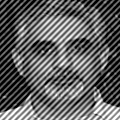
\includegraphics[width=.3\linewidth]{bossJailed1}&
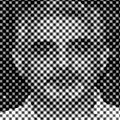
\includegraphics[width=.3\linewidth]{bossJailed2}&

\includegraphics[width=.3\linewidth]{mystery}
\\\textbf{bossJailed1.png} & \textbf{bossJailed2.png} & \textbf{mystery.png}
\end{tabular}

\item (\textbf{3 marks}) The abducters might have placed my boss in a maximum security prison as shown in \textbf{bossJailed2.png}. Can you free him from there too? Store the result in \textbf{bossFreed2.png}.

\item (\textbf{5 marks}) Impressed by your abilities to free captives, the abductors have challenged you to free a mystery captive in \textbf{mystery.png}. Can you free this captive as well? Who is the captive? Store the result in \textbf{Captive'sLastNameFreed.png}. You may use the code in the file \textbf{unjail\_manual.m} or \textbf{unjail.m} as you see fit.
\end{enumerate}

\newpage
\section*{Submission}
%This assignment is to be done in groups of 3 students each. \textbf{It is highly recommended that you try this assignment individually at first and then combine your results}. Email your assignment to the TA Nausheen Qaiser at \textbf{phdcsf13m005@pucit.edu.pk} as a .zip file with the naming convention

Paste your submission as a .zip file into the following folder on \textbackslash\textbackslash printsrv:
\begin{lstlisting}
\\printsrv\Teacher Data\Dr.Nazar Khan\Teaching\Fall2015\CS 565 Computer Vision\Submissions\Assignment2
\end{lstlisting}
Write access to this folder will be disabled after the submission deadline. The .zip file should have the following naming convention 
\begin{verbatim}
RollNumber_Assignment2.zip
\end{verbatim}
For example, if your roll number is MSCSF15M999, then the .zip file should be named \begin{verbatim}
MSCSF15M999_Assignment2.zip
\end{verbatim}
%\begin{verbatim}
%RollNumber1_RollNumber2_RollNumber3_YourName_Assignment2.zip
%\end{verbatim}
%For example, if roll numbers of your group members are BSEF11M997, BSEF11M998 and BSEF11M999,
%then the .zip file should be named
%\begin{verbatim}
%BSEF11M997_BSEF11M998_BSEF11M999_Assignment2.zip
%\end{verbatim}
The .zip file should contain the following directories:
\begin{itemize}
\item \textbf{Theoretical}
\item \textbf{Programming}
\end{itemize}
The \textbf{Theoretical} directory should contain the following:
\begin{enumerate}
\item A .txt/doc/pdf file called README.txt/doc/pdf containing your answers. If you want to write the answers by hand, then a digital photograph or scanned copy of your answers should be placed here.
\end{enumerate}
The \textbf{Programming} directory should contain the following:
\begin{enumerate}
\item The files 
\begin{enumerate}
\item \textbf{myAffineRescaling.m}
\item \textbf{myLogDynamicCompression.m}
\item \textbf{unjail\_manual.m}
\item \textbf{unjail.m}
\end{enumerate}
 supplemented with the missing code.
\item The images 
\begin{enumerate}
\item \textbf{bossFreed1.png},
\item \textbf{bossFreed2.png}, and
\item \textbf{Captive'sLastNameFreed.png}.
\end{enumerate}
\item A .txt file called README.txt describing how you managed to free all the captives. This should also include the identity of the mystery captive.
\end{enumerate}

\textbf{Please do not submit a very large .zip containing extra files. It should only contain what is asked for. If your .zip file contains any extra file(s), you will receive $0$ credit for the whole assignment.}

\textbf{Note}: To submit your results in a single, beautiful looking .pdf file, the La\TeX~source for this document is also provided in the Assignment2.tex file. You can use the command \textbackslash answer$\left\{\right\}$ to fill in your answers below each question. Please consult your instructor or TA for more help. \textbf{Remember: Word is ugly and La\TeX~is beautiful!}

\newpage

\begin{appendix}
\section{1D Discrete Fourier Transform}
The {\color{red}1D discrete Fourier transform} (DFT) of a \textbf{finite}, \textbf{sampled} signal $\mathbf{x} = (x_0, \dots, x_{M-1})^T$ with finite extent is given by
\begin{equation}
\hat{x}_u=\frac{1}{\sqrt{M}}\sum_{m=0}^{M-1}x_m e^{-i2\pi u \frac{m}{M}}
\end{equation}
for frequencies $u=(0,\dots,M-1)$.
A signal with $M$ values is decomposed into $M$ frequency coefficients.
The corresponding {\color{red}1D inverse discrete Fourier transform} is given by
\begin{equation}
x_m=\frac{1}{\sqrt{M}}\sum_{u=0}^{M-1}\hat{x}_ue^{i2\pi u \frac{m}{M}}
\end{equation}
for $m=(0,\dots,M-1)$.

\subsection{Interpretation as change of basis}
The Fourier basis is given by
\begin{equation}
\mathbf{f}_u=\frac{1}{\sqrt{M}}(e^{i2\pi u \frac{0}{M}},e^{i2\pi u \frac{1}{M}},\dots,e^{i2\pi u \frac{M-1}{M}})^T
\end{equation}
for frequencies $u=(0,\dots,M-1)$.
A signal $\mathbf{x}$ can be projected onto a basis vector $\mathbf{f}$ via the inner-product
\begin{equation}
<\mathbf{x},\mathbf{f}>=\sum_{m=0}^{M-1}x_m\bar{f}_m
\end{equation}
The DFT computes the Fourier basis coefficients $\hat{x}_u=<\mathbf{x},\mathbf{f}_u>$ for frequencies $u=(0,\dots,M-1)$.
The inverse DFT reconstructs the signal from the Fourier basis coefficients via $\mathbf{x}=\sum_{u=0}^{M-1}\hat{x}_u\mathbf{f}_u$.
\end{appendix}

\subsection{Proving orthogonality of Fourier basis vectors}
You might need the formula for the sum of a geometric series
\begin{equation}
\sum_{m=0}^{M-1}r^m=\frac{1-r^M}{1-r}
\end{equation}

\end{document}